% This file creates a document from a single lab.txt file
%
% It was set up 2023-3-22 by mgb to allow simple creation
% of a PDF for one lab. It's a copy of phsc12720-lab-manual
% with most content deleted or commented out.
%
% To get the correct lab number in the title, set the variable
% in the line below.
\def\labnumber{2}

\documentclass[answerkey]{msulabm}
\usepackage[utf8]{inputenc}
\usepackage{amsmath}
\usepackage{graphicx}
%\usepackage[linktocpage]{hyperref}  % if not using colorlinks, use linktocpage
\usepackage[colorlinks]{hyperref}  % if not using colorlinks, use linktocpage
\usepackage{bm}            % bold math
\usepackage{multirow}
\usepackage[table]{xcolor} % provide alternating rows with colors
\usepackage{textcomp}
\usepackage{xfrac} % gives split-level fractions with '\sfrac{a}{b}
\usepackage{multicol}
\usepackage[section]{placeins} % provides \FloatBarrier, to keep floats from crossing this barrier
\usepackage{amssymb}
\usepackage{wrapfig} % provides wrapping figures with text.
%\usepackage{enumitem} % gives \begin{enumerate}[resume] to resume counting from previous enumerate
%\usepackage{subfigure}
%\usepackage{tikz} % to draw arrows
\usepackage{xtab} % provides xtabular, tabular environment that spans multiple pages and other awesome things
\usepackage[style=phys,biblabel=brackets,pageranges=false]{biblatex}
\usepackage{pdflscape}
\usepackage{ragged2e}
\usepackage{longtable}
\usepackage{mathabx} % gives astronomy symbols like \Earth
\usepackage{pdfpages}
\usepackage{wasysym}

\bibliography{../references-manual,../bbarker-zotero}



\newcommand{\abs}[1]{\left\lvert#1\right\rvert}

%\title{Laboratory Manual}
%\author{PHSC 12620 Big Bang \\ \\ The University of Chicago}
%\date{Spring 2023}

\pagestyle{ruled}

\definecolor{lgray}{rgb}{.2,.2,.2}

\makeevenfoot{ruled}{\thepage}{\footnotesize{\textit{Last updated \today}}}{}
%\makeevenfoot{ruled}{\thepage}{}}{}
\makeoddfoot{ruled}{}{\color{lgray} \tiny{This work is licensed under \href{http://creativecommons.org/licenses/by-sa/4.0/}{CC BY-SA 4.0} by \href{mailto:bbarker@uchicago.edu}{the University of Chicago}.}}{\thepage}


% allows us to use subcaptions from the memoir class in figures. See Memoir Section 10.9
\newsubfloat{figure}

% don't worry so much about filling every page.
%\raggedbottom

% raise the penalty for splitting footnotes across different pages. Default is 100.
\interfootnotelinepenalty=10000

%\includeonly{amplifier/amplifier} 

% creates a standard length to use 
\newlength{\answerskip}
%\setlength{\answerskip}{90pt} 

%% use plus / minus if latex is squeezing the answer space too much
\setlength{\answerskip}{2cm plus 0.2cm minus 0.2cm}

\newlength{\qaskip}
\setlength{\qaskip}{\answerskip}
\addtolength{\qaskip}{\baselineskip}

% reduce vertical space between chapters in table of contents. Default is 2em.
\setlength{\cftbeforechapterskip}{1em}

% allow for extra line on a page to help prevent widow/orphan lines.
\sloppybottom

% Now we can caption a table outside of the table float environment (good for multi-page tables)
\newfixedcaption{\freetabcaption}{table}

%\includeonly{snells-law/snells-law}
%\includeonly{ohms-law/ohms-law}

\begin{document}
\maxtocdepth{chapter}

% start roman numbering
%\frontmatter

%\maketitle

%\clearpage

%Brent W. Barker

%Department of Astronomy \& Astrophysics

%The University of Chicago

%5640 South Ellis Ave.

%Chicago, IL 60637

%\href{mailto:bbarker@uchicago.edu}{bbarker@uchicago.edu}

%\vspace{2\baselineskip}

%\includegraphics{cc-by-sa-88x31}

%\textcopyright{} 2018 Brent W. Barker. Except where otherwise noted, this work is copyrighted under the Creative Commons Attribution-ShareAlike International 4.0 License. To view a copy of this license, visit \url{http://creativecommons.org/licenses/by-sa/4.0/}.

%\vspace{\baselineskip}

%These labs, excluding "Impulse and Momentum" and the appendices, are a derivative of "\href{https://%sites.google.com/site/scientificabilities/ISLE-labs}{ISLE Labs}" by the Rutgers Physics and Astronomy %Education Research group, used under the Creative Commons Attribution International 4.0 License.
%To view a copy of this license, visit \url{http://creativecommons.org/licenses/by/4.0/}.

%At Rutgers University, many people contributed to this project over the years.
%The list of names is very long and includes: Eugenia Etkina, Alan Van Heuvelen, Suzanne Brahmia, David %Brookes, Michael Gentile, Anna Karelina, Michael Lawrence, Marina Milner-Bolotin, Sahana Murthy, Maria %Ruibal-Villasenor, Aaron Warren, Xueli Zou.

% skip to next right leaf (``recto'')
%\cleartorecto

 % the star means that the ToC itself is not listed in the ToC
 %\tableofcontents*

 % start arabic numbering
%\mainmatter 

\setcounter{chapter}{\labnumber-1} % Set this to (Lab Number)-1
\chapter{Galactic distances and the Hubble diagram}

%todo remove a couple galaxies - some are especially difficult to see the Ca lines with. framing: students need to judge what to do in this case --- sometimes data is not reliable.

%todo rewrite to have students need to design a procedure to find angular separation of galaxies

%todo cannot see coordinates of cursor in Google Chrome. Works in Firefox and Safari (2022).

\section{Introduction}

In 1929, Edwin Hubble measured that distant galaxies were
systematically redshifted relative to galaxies that were closer. From this
data, Hubble inferred that the universe was expanding, an idea initially
worked out by Georges Lemaitre using Einstein's theory of gravity.

In this lab, you will conduct a measurement similar to Hubble's and will
produce your own version of his famous Hubble diagram shown below.

\section{Team roles}

\textbf{Decide on roles} for each group member. The available roles are:

\begin{itemize}
	\item Facilitator: ensures time and group focus are efficiently used
	\item Scribe: ensures work is recorded
	\item Technician: oversees apparatus assembly, usage
	\item Skeptic: ensures group is questioning itself
\end{itemize}

These roles can rotate each lab, and you will report at the end of the lab report on how it went for each role. If you have fewer than 4 people in your group, then some members will be holding more than one role. For example, you could have the skeptic double with another role. Consider taking on a role you are less comfortable with, to gain experience and more comfort in that role.

Additionally, if you are finding the lab roles more restrictive than helpful, you can decide to co-hold some or all roles, or think of them more like functions that every team needs to carry out, and then reflecting on how the team executed each function.

\begin{steps}
	\item On Canvas, navigate to the People section, then to the ``L2 Hubble'' tab. Find a group that is not yet used, and have each person in your group add themselves to that same lab group.
\end{steps}

\section{Building intuition}

The graph in Figure~\ref{hd:fig:hubble-diagram-schematic} illustrates the impact of an expanding universe of
photons emitted from distant objects. Because the speed of light is
constant, photons that we measure today were emitted in the past, with
photons originating from objects that are further away being emitted
earlier in time. This means that photons from objects that are further
away are older, and thus, those photons have experienced more expansion by the universe.

\begin{figure}
	\centering
	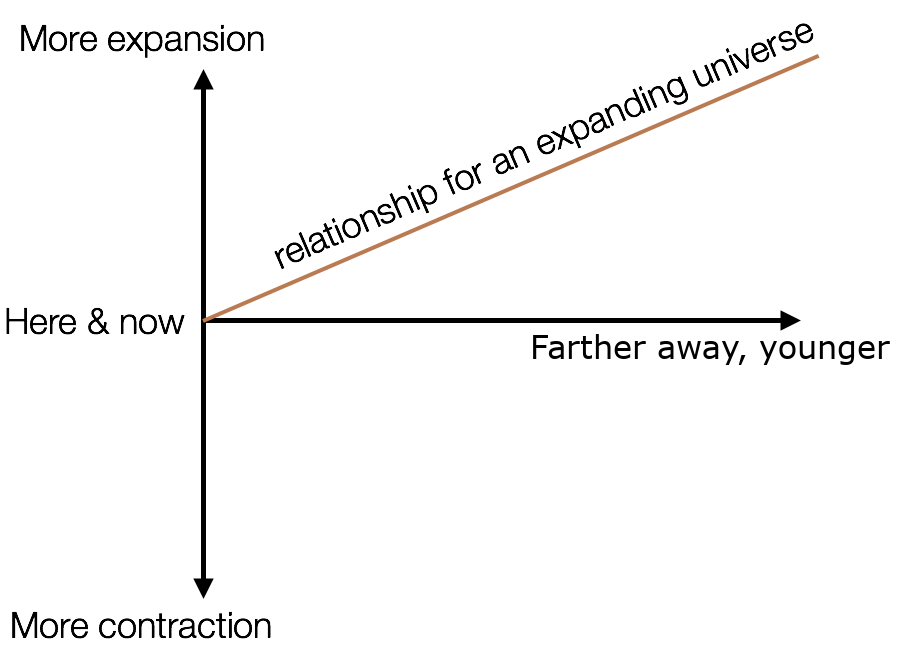
\includegraphics[width=0.5\textwidth]{hubble-diagram/hubble-diagram-schematic}
	\caption{Schematic of a Hubble diagram plot. It illustrates the relationship between the expansion
		experienced by a photon and the distance of its emitter.}\label{hd:fig:hubble-diagram-schematic}
\end{figure}

\begin{steps}
	\item\label{hd:step:sketch} Sketch the plot from Figure~\ref{hd:fig:hubble-diagram-schematic}, then sketch on the plot two more lines corresponding to the
	relationship for 1) a contracting universe, and 2) a static universe.
\end{steps}

From this relationship, we can determine whether the universe is
expanding, contracting, or static by looking at a number of galaxies and
measuring their distance (corresponding to the horizontal axis) and the
expansion experienced by their photons (corresponding to the vertical axis).

For this lab, we will use galaxy images and spectra listed in an online
table.

\section{Measuring distance}

We will use geometry to measure the distance of our galaxies. Galaxies
that are closer will look bigger and will subtend a larger angle whereas
galaxies that are further will looks smaller and will subtend a smaller
angle. This relationship between the angular size of the galaxy and its
distance is illustrated in Figure~\ref{hd:fig:galaxy-subtend}.

\begin{figure}
	\centering
	\includegraphics[width=\textwidth]{hubble-diagram/galaxy-subtend}
	\caption{Looking from the dot on the left, there are two galaxies that are the same size, one further away than the other. The more distant galaxy subtends a smaller angle (dashed green lines) than the closer galaxy (solid red lines).}\label{hd:fig:galaxy-subtend}
\end{figure}

Our galaxies will all be nearly the same size (22 kpc). Using the
geometry shown in the illustration, we can arrive at the following
relationship:
\begin{equation}\label{hd:eq:size}
 \textrm{angular size} = \frac{22\:\textrm{kpc}}{\textrm{distance}} \,.
\end{equation}
So, by measuring the angular size of our galaxy images, we can use the
above equation to determine the distance to the galaxy.

From the Modules $>$ Lab section of the Canvas site, download and extract to a folder \texttt{HubbleDataWebpage.zip}. In that folder, open \texttt{HubbleDataPage.html}. You
will find a list of galaxy names. Click on the ``Image'' link for the first
galaxy, NGC 1357. In the new tab, you will see an image of galaxy NGC
1357 similar to Figure~\ref{hd:fig:galaxy-example}.

\begin{figure}
	\centering
	\includegraphics[width=0.5\textwidth]{hubble-diagram/galaxy-example}
	\caption{Example of galaxy image. Colors are inverted here, and Points 1 and 2 mark the furthest extent of the galaxy}\label{hd:fig:galaxy-example}
\end{figure}

\begin{steps}
	\item\label{hd:step:kind} What kind of galaxy is it (spiral, elliptical, unclear)? Note this in your spreadsheet.
	
	\item Are there any noteworthy features in the image? Use your spreadsheet to record your answers.
\end{steps}

We want to measure the angular size of NGC 1357, which you can do by
measuring the angular separation between two appropriate points
spanning the entire galaxy. In the lower left hand corner of google
skymaps, google shows you the coordinates of your cursor. Record the
coordinates (RA and DEC) for two points spanning the galaxy. Then use
an online calculator (e.g.
\url{http://cads.iiap.res.in/tools/angularSeparation}) to calculate the
angular separation between the points. Be careful and make sure that you don’t choose points that are too far
outside or inside the galaxy image.

\begin{steps}
	\item\label{hd:step:size} Enter the value for the angular size
(in radians, not degrees) in a spreadsheet.

	\item Divide up the remaining galaxy images between your groupmates
	and repeat Steps~\ref{hd:step:kind}--\ref{hd:step:size} for each of the galaxies recording your notes
	and measurements in the spreadsheet.
	
	\item Once you have measured the angular size of all the galaxies, use Equation~\ref{hd:eq:size} to estimate the distance for each galaxy
	and record the values in a “distance” column.
\end{steps}





\section{Measuring expansion}

The wavelength of light changes as the universe expands, an effect
known as cosmological redshifting. If the universe expands, the
wavelength is stretched, becoming longer and redder. For a contracting
universe, the wavelength will be compressed becoming bluer. We define
the redshift, $z$, as
\begin{equation}\label{hd:eq:redshift}
 z = \frac{\lambda_\textrm{measured} - \lambda_\textrm{original}}{\lambda_\textrm{original}} \,,
\end{equation}
where $\lambda$ represents the wavelength. The redshift is a measure of how much the wavelength has been
stretched or compressed.

We can measure the redshift by examining spectra (the energy emitted
in different wavelengths) of the same galaxies we just measured. For
NGC 1357, click on the link “Ca Spectra.” The link will show spectra
associated with Ca absorption which produces dips at wavelengths of
3933.7 angstroms and 3968.5 angstroms. You should see two
prominent dips in the data. See Figure~\ref{hd:fig:spectra} for example spectra.

\begin{figure}
	\centering
	\includegraphics[width=\textwidth]{hubble-diagram/spectra}
	\caption{Spectrum of light detected from NGC 1357. The dips and peak that you will use to identify redshift are identified.}\label{hd:fig:spectra}
\end{figure}

Go back to the galaxy list and click on the
link “H-alpha spectrum” to bring up the spectra associated with
Hydrogen alpha emission of light with wavelength 6562.8 Angstroms.
You should see a clear peak in the data. The H-alpha peak is the leftmost
of the distribution. Since we know the original wavelengths for these
processes, we can compare the measured wavelength of these features
with their original wavelength to determine how much the light has
stretched.

\begin{steps}
	\item For each of the spectra estimate the value for the two Ca dips and the H-alpha peak. Record the values for the two Ca absorption lines and the H-alpha emission line in the excel worksheet. 
	
	\item Use Equation~\ref{hd:eq:redshift} to calculate the redshift for each of the lines and take the average to
estimate the redshift for the galaxy. Record the redshift in an “average
redshift” column in the spreadsheet.

	\item Repeat this process for each of
your galaxies.
\end{steps}

%\section{Compare your measurements}
%
%Compile the data between you and your groupmates into a single table.
%Compare your values for distance and redshift with those obtained by
%other groups in your section.
%
%\begin{steps}
%	\item How well do your data agree?
%	
%	\item Are they consistently different? If so, what do you think leads to
%	this discrepancy?
%	
%	\item Do they differ in a random fashion? If so, do they differ a lot or a
%	little? Provide your reasoning for your assessment.
%\end{steps}

\section{The Hubble diagram}

\begin{steps}
	
	\item Using the measurements in your worksheet, make a plot of redshift
	versus distance for your galaxies.
	
	\item Is there a trend in your data? Is the trend clear?
	
	\item Compare your plot with the sketches from Step~\ref{hd:step:sketch}. Does your data
	indicate that the universe is expanding? Contracting? Static? Why?

\end{steps}

Hubble's constant $H_0$ gives a relation between the recessional speed $v$ of an object and its distance $D$, according to the equation
\begin{equation}\label{hd:eq:hubble}
 v = H_0 D \,.
\end{equation}
You will determine Hubble's constant from your data. You have the distances of the galaxies already. To find the velocities, multiply the redshift by the speed of light $c$,
\begin{equation}
 v = zc \,.
\end{equation}
This equation is valid for low values of redshift.

\begin{steps}
	
	\item Make a Hubble diagram by plotting velocity (in km/s) vs. distance (in Mpc).
	
	\item Use this plot and Equation~\ref{hd:eq:hubble} to fit a line to the data and find Hubble's constant, which should be the slope of that line. If you are doing a linear fit, you need to force the $y$-intercept of the line to be zero. You may also need to specify that the fit equation be displayed on the plot.
	
	\item Do some research on the history and background of Hubble’s
	measurement. Write a one paragraph summary of this lab and discuss
	the following:
	\begin{enumerate}
		\item What was the historical context of Hubble’s measurement?
		\item Why was it important?
		\item What did you do in this lab and how do your measurements and
		conclusions compare with Hubble’s?
	\end{enumerate}
\end{steps}

\section{Report checklist and grading}

%Include the following in your lab report. See Appendix~\ref{cha:lab-report-format} for formatting details. Each item below is worth 10 points.
Include the following in your lab report. See Appendix~A for formatting details. Each item below is worth 10 points.

\begin{enumerate}
	\item Data table
	
	\item Sketch of predicted relations for expanding, contracting, and static universes
	
	\item Your Hubble diagram (velocity vs. distance)
	
	\item Your Hubble constant
	
	\item Answers to Questions 12, 13, and 16.
	
	\item Write a 100--200 word reflection on group dynamics. Address the following topics: who did what in the lab, how did you work together, how group roles functioned, what successes and challenges in group functioning did you have, and what might you want to do differently next time?
\end{enumerate}


%\appendix
%\include{report-format-short/report-format-short}
%\chapter{Analysis of Uncertainty}\label{cha:uncertainty}

%todo mark std dev equation and general error propagation formula as optional/advanced - recommend use =STDDEV to compute

A physical quantity consists of a value, unit, and uncertainty.
For example, ``$5 \pm 1\,$m'' means that the writer believes the true value of the quantity to most likely lie within 4 and 6 meters\footnote{The phrase ``most likely'' can mean different things depending on who is writing.
	If a physicist gives the value and does not given a further explanation, we can assume that they mean that the measurements are randomly distributed according to a normal distribution around the value given, with a standard deviation of the uncertainty given.
	So if one were to make the same measurement again, the author believes it has a 68\% chance of falling within the range given.
	Disciplines other than physics may intend the uncertainty to be 2 standard deviations.}.
Without knowing the uncertainty of a value, the quantity is next to useless.
For example, in our daily lives, we use an implied uncertainty.
If I say that we should meet at around 5:00 pm, and I arrive at 5:05 pm, you will probably consider that within the range that you would expect.
Perhaps your implied uncertainty is plus or minus 15 minutes.
On the other hand, if I said that we would meet at 5:07 pm, then if I arrive at 5:10 pm, you might be confused, since the implied uncertainty of that time value is more like 1 minute.

Scientists use the mathematics of probability and statistics, along with some intuition, to be precise and clear when talking about uncertainty, and it is vital to understand and report the uncertainty of quantitative results that we present.

\section{Types of measurement uncertainty}\label{unc:sec:types}

For simplicity, we limit ourselves to the consideration of two types of uncertainty in this lab course, instrumental and random uncertainty.

\subsection{Instrumental uncertainties}

Every measuring instrument has an inherent uncertainty that is determined by the precision	
  of the instrument.
Usually this value is taken as a half of the smallest increment of the instrument's scale. For example, $0.5\:$mm is the precision of a standard metric ruler; $0.5\:$s is the precision of a watch, etc. For electronic digital displays, the equipment's manual often gives the instrument's resolution, which may be larger than that given by the rule above.

Instrumental uncertainties are the easiest ones to estimate, but they are not the only source of the uncertainty in your measured value.
You must be a skillful experimentalist to get rid of all other sources of uncertainty so that all that is left is instrumental uncertainty.

\subsection{Random uncertainties}\label{unc:random}

Very often when you measure the same physical quantity multiple times, you can get different results each time you measure it.
That happens because different uncontrollable factors affect your results randomly.
This type of uncertainty, random uncertainty, can be estimated only by repeating the same measurement several times.
For example if you measure the distance from a cannon to the place where the fired cannonball hits the ground, you could get different distances every time you repeat the same experiment.	
  
For example, say you took three measurements and obtained 55.7, 49.0, 52.5, 42.4, and 60.2 meters. We can quantify the variation in these measurements by finding their standard deviation using a calculator, spreadsheet (like Microsoft Excel, LibreOffice Calc, or Google Sheets), or the formula (assuming the data distributed according to a normal distribution)
\begin{equation}
 \sigma = \sqrt{\sum_{i=1}^{N} \frac{(x_i-\bar{x})^2}{N-1}} \, ,
\end{equation}
where $\{x_1, x_2, \dots, x_N\}$ are the measured values, $\bar{x}$ is the mean of those values, and $N$ is the number of measurements.
For our example, the resulting standard deviation is 6.8 meters. Generally we are interested not in the variation of the measurements themselves, but how uncertain we are of the average of the measurements. The uncertainty of this mean value is given, for a normal distribution, by the so-called ``standard deviation of the mean'', which can be found by dividing the standard deviation by the square root of the number of measurements,
\begin{equation}\label{unc:eq:stdevmean}
\sigma_\textrm{mean} = \frac{\sigma}{\sqrt{N}} \, .
\end{equation}
So, in this example, the uncertainty of the mean is 3.0 meters. We can thus report the length as $52 \pm 3\:$m.

Note that if we take more measurements, the standard deviation of those measurements will not generally change, since the variability of our measurements shouldn't change over time. However, the standard deviation of the mean, and thus the uncertainty, will decrease.

\section{Propagation of uncertainty}\label{unc:sec:prop}

When we use an uncertain quantity in a calculation, the result is also uncertain. To determine by how much, we give some simple rules for basic calculations, and then a more general rule for use with any calculation which requires knowledge of calculus. Note that these rules are strictly valid only for values that are normally distributed, though for the purpose of this course, we will use these formulas regardless of the underlying distributions, unless otherwise stated, for simplicity.

If the measurements are completely independent of each other, then for quantities $a \pm \delta a$ and $b \pm \delta b$, we can use the following formulas:
\begin{equation}\label{unc:add}
\textrm{For } c = a + b \textrm{ (or for subtraction), } \delta c = \sqrt{(\delta a)^2 + (\delta b)^2}
\end{equation}

\begin{equation}\label{unc:mult}
\textrm{For } c = ab \textrm{ (or for division), } \frac{\delta c}{c} = \sqrt{\left(\frac{\delta a}{a}\right)^2 + \left(\frac{\delta b}{b}\right)^2}
\end{equation}

\begin{equation}\label{unc:exp}
\textrm{For } c = a^n,\, \frac{\delta c}{c} = n \frac{\delta a}{a}
\end{equation}

For other calculations, there is a more general formula not discussed here.

%If you are familiar with calculus, you may want to use this general formula for the uncertainty $\delta f$ of a function $f$ of $N$ independent values $x_i$, each with uncertainty $\delta x_i$:
%\begin{equation}\label{unc:general}
%\delta f = \sqrt{ \sum_{i=1}^{N} \left(\frac{\partial f}{\partial x_i} \delta x_i\right)^2 } \, .
%\end{equation}
%Notice that Eqs.\ \ref{unc:add} through \ref{unc:exp} can be derived from Eq.\ \ref{unc:general} for those specific cases.

\subsubsection{What if there is no reported uncertainty?}

Sometimes you'll be calculating with numbers that have no uncertainty given.
In some cases, the number is exact.
For example, the circumference $C$ of a circle is given by $C = 2 \pi r$. Here, the coefficient, $2\pi$, is an exact quantity and you can treat its uncertainty as zero.
If you find a value that you think is uncertain, but the uncertainty is not given, a good rule of thumb is to assume that the uncertainty is half the right-most significant digit.
So if you are given a measured length of $1400\:$m, then you might assume that the uncertainty is $50\:$m.
This is an assumption, however, and should be described as such in your lab report.
For more examples, see Table~\ref{unc:tab:implied}.

\begin{table}
	\begin{center}
		\begin{tabular}{cc}
			\textbf{Expression} & \textbf{Implied uncertainty} \\
			12 & 0.5 \\
			12.0 & 0.05 \\
			120 & 5 \\
			120. & 0.5
		\end{tabular}
		\caption{Expression of numbers and their implied uncertainty.}\label{unc:tab:implied}
	\end{center}
\end{table}

\subsubsection{How many digits to report?}

After even a single calculation, a calculator will often give ten or more digits in an answer.
For example, if I travel $11.3 \pm 0.1\:$km in $350 \pm 10\:$s, then my average speed will be the distance divided by the duration. Entering this into my calculator, I get the resulting value ``\texttt{0.0322857142857143}''.
Perhaps it is obvious that my distance and duration measurements were not precise enough for all of those digits to be useful information.
We can use the propagated uncertainty to decide how many decimals to include.
Using the formulas above, I find that the uncertainty in the speed is given by my calculator as ``\texttt{9.65683578099600e-04}'', where the `\texttt{e}' stands for ``times ten to the''.
I definitely do not know my uncertainty to 14 decimal places.
For reporting uncertainties, it general suffices to use just the 1 or 2 left-most significant digits, unless you have a more sophisticated method of quantifying your uncertainties.
So here, I would round this to 1 significant digit, resulting in an uncertainty of $0.001\:$km/s.
Now I have a guide for how many digits to report in my value.
Any decimal places to the right of the one given in the uncertainty are distinctly unhelpful, so I report my average speed as ``$0.032 \pm 0.001\:$km/s''.
You may also see the equivalent, more succinct notation ``$0.032(1)\:$km/s''.

\section{Comparing two values}\label{unc:sec:comparing}

If we compare two quantities and want to find out how different they are from each other, we can use a measure we call a $t'$ value (pronounced ``tee prime''). This measure is not a standard statistical measure, but it is simple and its meaning is clear for us.

Operationally, for two quantities having the same unit, $a \pm \delta a$ and $b \pm \delta b$, the measure is defined as\footnote{Statistically, if $\delta a$ and $\delta b$ are uncorrelated, random uncertainties, then $t'$ represents how many standard deviations the difference $a - b$ is away from zero.}

\begin{equation}
%t' = \frac{\abs{a-b}}{\sqrt{(\delta a)^2 + (\delta b)^2}}
t' = \frac{\abs{a-b}}{\sqrt{(\delta a)^2 + (\delta b)^2}}
\end{equation}

If $t' \lesssim 1$, then the values are so close to each other that they are indistinguishable. It is either that they represent the same true value, or that the measurement should be improved to reduce the uncertainty.

If $1 \lesssim t' \lesssim 3$, then the result is inconclusive. One should improve the experiment to reduce the uncertainty.

If $t' \gtrsim 3$, then the true values are very probably different from each other.
%
\chapter{Rubrics}\label{cha:rubrics}

%Each lab is graded 50\% on attendance and participation during the lab, and providing evidence in the lab report of completing all steps of the lab, including answering every question. The other 50\% is based on a selection of scientific abilities.

%Each scientific ability rubric row assessed is worth a possible 1 point, with ``Missing'' being 0 points, ``Inadequate'' 1/3 points, ``Needs Improvement'' 2/3 points, and ``Adequate'' 1 point.

The scientific abilities rubrics are found on the following pages.

\begin{landscape}

\begin{longtable}{>{\bfseries}p{0.04\textheight}|>{\bfseries\RaggedRight}p{0.23\textheight}|>{\RaggedRight}p{0.21\textheight}|>{\RaggedRight}p{0.21\textheight}|>{\RaggedRight}p{0.22\textheight}|>{\RaggedRight}p{0.22\textheight}}
	\toprule
	& Scientific Ability
	& Missing & Inadequate & Needs Improvement & Adequate \\ \midrule \endhead
	A11
	& Graph
	& No graph is present.
	& A graph is present but the axes are not labeled. There is no scale on the axes.
	& The graph is present and axes are correctly labeled, but the axes do not correspond to the independent and dependent variables, or the scale is not accurate.
	& The graph has correctly labeled axes, independent variable is along the horizontal axis and the scale is accurate.
	\\
	\bottomrule
	\caption{Rubric A: Ability to represent information in multiple ways}\label{rubric:a}
	\end{longtable}

\begin{longtable}{>{\bfseries}p{0.02\textheight}|>{\bfseries\RaggedRight}p{0.25\textheight}|>{\RaggedRight}p{0.21\textheight}|>{\RaggedRight}p{0.21\textheight}|>{\RaggedRight}p{0.22\textheight}|>{\RaggedRight}p{0.22\textheight}}
		\toprule
		& Scientific Ability
		& Missing & Inadequate & Needs Improvement & Adequate \\ \midrule \endhead
		B1
		& Is able to identify the phenomenon to be investigated
		& No phenomenon is mentioned
		& The description of the phenomenon to be investigated is confusing, or it is not the phenomenon of interest.
		& \midsloppy The description of the phenomenon is vague or incomplete.
		& The phenomenon to be investigated is clearly stated. \\ \midrule
		B2
		& Is able to design a reliable experiment that investigates the phenomenon
		& The experiment does not investigate the phenomenon.
		& The experiment may not yield any interesting patterns.
		& Some important aspects of the phenomenon will not be observable.
		& The experiment might yield interesting patterns relevant to the investigation of the phenomenon. \\ \midrule
		B3
		& Is able to decide what physical quantities are to be measured and identify independent and dependent variables
		& The physical quantities are irrelevant.
		& Only some of physical quantities are relevant.
		& The physical quantities are relevant. However, independent and dependent variables are not identified.
		& The physical quantities are relevant and independent and dependent variables are identified. \\ \midrule
		B4
		& Is able to describe how to use available equipment to make measurements
		& At least one of the chosen measurements cannot be made with the available equipment.
		& All chosen measurements can be made, but no details are given about how it is done.
		& All chosen measurements can be made, but the details of how it is done are vague or incomplete.
		& All chosen measurements can be made and all details of how it is done are clearly provided. \\ \midrule
		B5
		& Is able to describe what is observed without trying to explain, both in words and by means of a picture of the experimental setup
		& No description is mentioned.
		& A description is incomplete. No labeled sketch is present. Or, observations are adjusted to fit expectations.
		& A description is complete, but mixed up with explanations or pattern. Or the sketch is present but is difficult to understand.
		& Clearly describes what happens in the experiments both verbally and with a sketch. Provides other representations when necessary (tables and graphs). \\ \midrule
		B6
		& Is able to identify the shortcomings in an experiment and suggest improvements
		& No attempt is made to identify any shortcomings of the experiment.
		& The shortcomings are described vaguely and no suggestions for improvement are made.
		& Not all aspects of the design are considered in terms of shortcomings or improvements.
		& All major shortcomings of the experiment are identified and reasonable suggestions for improvement are made. \\ \midrule
		B7
		& Is able to identify a pattern in the data
		& No attempt is made to search for a pattern.
		& The pattern described is irrelevant or inconsistent with the data.
		& The pattern has minor errors or omissions. Terms like ``proportional'' used without clarity, e.g.\ is the proportionality linear, quadratic, etc.
		& The pattern represents the relevant trend in the data. When possible, the trend is described in words. \\ \midrule
		B8
		& Is able to represent a pattern mathematically (if applicable)
		& No attempt is made to represent a pattern mathematically.
		& The mathematical expression does not represent the trend.
		& No analysis of how well the expression agrees with the data is included, or some features of the pattern are missing.
		& The expression represents the trend completely and an analysis of how well it agrees with the data is included. \\ \midrule
		B9
		& Is able to devise an explanation for an observed pattern
		& No attempt is made to explain the observed pattern.
		& An explanation is vague, not testable, or contradicts the pattern.
		& An explanation contradicts previous knowledge or the reasoning is flawed.
		& A reasonable explanation is made. It is testable and it explains the observed pattern. \\
		\bottomrule
		\caption{Rubric B: Ability to design and conduct an observational experiment \cite{etkina_scientific_2006}.}\label{rubric:b}
	\end{longtable}

\begin{longtable}{>{\bfseries}p{0.02\textheight}|>{\bfseries\RaggedRight}p{0.25\textheight}|>{\RaggedRight}p{0.21\textheight}|>{\RaggedRight}p{0.21\textheight}|>{\RaggedRight}p{0.22\textheight}|>{\RaggedRight}p{0.22\textheight}}
	\toprule
	& Scientific Ability
	& Missing & Inadequate & Needs Improvement & Adequate \\ \midrule \endhead
	C1
	& Is able to identify the hypothesis to be tested
	& No mention is made of a hypothesis.
	& An attempt is made to identify the hypothesis to be tested but it is described in a confusing manner.
	& The hypothesis to be tested is described but there are minor omissions or vague details.
	& The hypothesis is clearly, specifically, and thoroughly stated.
	\\ \midrule
	C2
	& Is able to design a reliable experiment that tests the hypothesis
	& The experiment does not test the hypothesis.
	& The experiment tests the hypothesis, but due to the nature of the design it is likely the data will lead to an incorrect judgment.
	& The experiment tests the hypothesis, but due to the nature of the design there is a moderate chance the data will lead to an inconclusive judgment.
	& The experiment tests the hypothesis and has a high likelihood of producing data that will lead to a conclusive judgment.
	\\ \midrule
	C4
	& Is able to make a reasonable prediction based on a hypothesis
	& No prediction is made. The experiment is not treated as a testing experiment.
	& A prediction is made, but it is identical to the hypothesis, OR prediction is made based on a source unrelated to the hypothesis being tested, or is completely inconsistent with hypothesis being tested, OR prediction is unrelated to the context of the designed experiment.
	& Prediction follows from hypothesis but is flawed because relevant assumptions are not considered, OR prediction is incomplete or somewhat inconsistent with hypothesis, OR prediction is somewhat inconsistent with the experiment.
	& A prediction is made that follows from hypothesis, is distinct from the hypothesis, accurately describes the expected outcome of the experiment, and incorporates relevant assumptions if needed.
	\\ \midrule
	C5
	& Is able to identify the assumptions made in making the prediction
	& No attempt is made to identify assumptions.
	& An attempt is made to identify assumptions, but the assumptions are irrelevant or are confused with the hypothesis.
	& Relevant assumptions are identified but are not significant for making the prediction.
	& Sufficient assumptions are correctly identified, and are significant for the prediction that is made.
	\\ \midrule
	C6
	& Is able to determine specifically the way in which assumptions might affect the prediction
	& No attempt is made to determine the effects of assumptions.
	& The effects of assumptions are mentioned but are described vaguely.
	& The effects of assumptions are determined, but no attempt is made to validate them.
	& The effects of assumptions are determined and the assumptions are validated.
	\\ \midrule
	C7
	& Is able to decide whether the prediction and the outcome agree/disagree
	& No mention of whether the prediction and outcome agree/disagree.
	& A decision about the agreement/disagreement is made but is not consistent with the results of the experiment.
	& A reasonable decision about the agreement/disagreement is made but experimental uncertainty is not taken into account.
	& A reasonable decision about the agreement/disagreement is made and experimental uncertainty is taken into account.
	\\ \midrule
	C8
	& Is able to make a reasonable judgment about the hypothesis
	& No judgment is made about the hypothesis.
	& A judgment is made but is not consistent with the outcome of the experiment.
	& A judgment is made, is consistent with the outcome of the experiment, but assumptions are not taken into account.
	& A judgment is made, is consistent with the outcome of the experiment, and assumptions are taken into account.
	\\ \bottomrule
	\caption{Rubric C: Ability to design and conduct a testing experiment \cite{etkina_scientific_2006}.}\label{rubric:c}
\end{longtable}

\begin{longtable}{>{\bfseries}p{0.02\textheight}|>{\bfseries\RaggedRight}p{0.25\textheight}|>{\RaggedRight}p{0.21\textheight}|>{\RaggedRight}p{0.21\textheight}|>{\RaggedRight}p{0.22\textheight}|>{\RaggedRight}p{0.22\textheight}}
	\toprule
	& Scientific Ability
	& Missing & Inadequate & Needs Improvement & Adequate \\ \midrule \endhead
	D1
	& Is able to identify the problem to be solved
	& No mention is made of the problem to be solved.
	& An attempt is made to identify the problem to be solved but it is described in a confusing manner.
	& The problem to be solved is described but there are minor omissions or vague details.
	& The problem to be solved is clearly stated.
	\\ \midrule
	D2
	& Is able to design a reliable experiment that solves the problem.
	& The experiment does not solve the problem.
	& The experiment attempts to solve the problem but due to the nature of the design the data will not lead to a reliable solution.
	& The experiment attempts to solve the problem but due to the nature of the design there is a moderate chance the data will not lead to a reliable solution.
	& The experiment solves the problem and has a high likelihood of producing data that will lead to a reliable solution.
	\\ \midrule
	D3
	& Is able to use available equipment to make measurements
	& At least one of the chosen measurements cannot be made with the available equipment.
	& All of the chosen measurements can be made, but no details are given about how it is done.
	& All of the chosen measurements can be made, but the details about how they are done are vague or incomplete.
	& All of the chosen measurements can be made and all details about how they are done are provided and clear.
	\\ \midrule
	D4
	& Is able to make a judgment about the results of the experiment
	& No discussion is presented about the results of the experiment.
	& A judgment is made about the results, but it is not reasonable or coherent.
	& An acceptable judgment is made about the result, but the reasoning is incomplete, OR uncertainties are not taken into account, OR assumptions are not discussed, OR the result is written as a single number.
	& An acceptable judgment is made about the result, with clear reasoning. The effects of assumptions and experimental uncertainties are considered. The result is written as an interval.
	\\ \midrule
	D5
	& Is able to evaluate the results by means of an independent method
	& No attempt is made to evaluate the consistency of the result using an independent method.
	& A second independent method is used to evaluate the results. However there is little or no discussion about the differences in the results due to the two methods.
	& A second independent method is used to evaluate the results. The results of the two methods are compared correctly using experimental uncertainties. But there is little or no discussion of the possible reasons for the differences when the results are different.
	& A second independent method is used to evaluate the results and the evaluation is correctly done with the experimental uncertainties. The discrepancy between the results of the two methods, and possible reasons are discussed.
	\\ \midrule
	D7
	& Is able to choose a productive mathematical procedure for solving the experimental problem
	& Mathematical procedure is either missing, or the equations written down are irrelevant to the design.
	& A mathematical procedure is described, but is incorrect or incomplete, due to which the final answer cannot be calculated. Or units are inconsistent.
	& Correct and complete mathematical procedure is described but an error is made in the calculations. All units are consistent.
	& Mathematical procedure is fully consistent with the design. All quantities are calculated correctly with proper units. Final answer is meaningful.
	\\ \midrule
	D8
	& Is able to identify the assumptions made in using the mathematical procedure
	& No attempt is made to identify any assumptions.
	& An attempt is made to identify assumptions, but the assumptions are irrelevent or incorrect for the situation.
	& Relevant assumptions are identified but are not significant for solving the problem.
	& All relevant assumptions are correctly identified.
	\\ \midrule
	D9
	& Is able to determine specifically the way in which assumptions might affect the results
	& No attempt is made to determine the effects of assumptions.
	& The effects of assumptions are mentioned but are described vaguely.
	& The effects of assumptions are determined, but no attempt is made to validate them.
	& The effects of assumptions are determined and the assumptions are validated.
	\\ \bottomrule
	\caption{Rubric D: Ability to design and conduct an application experiment \cite{etkina_scientific_2006}.}\label{rubric:d}
\end{longtable}

\begin{longtable}{>{\bfseries}p{0.02\textheight}|>{\bfseries\RaggedRight}p{0.25\textheight}|>{\RaggedRight}p{0.21\textheight}|>{\RaggedRight}p{0.21\textheight}|>{\RaggedRight}p{0.22\textheight}|>{\RaggedRight}p{0.22\textheight}}
	\toprule
	& Scientific Ability
	& Missing & Inadequate & Needs Improvement & Adequate \\ \midrule \endhead	
	F1
	& Is able to communicate the details of an experimental procedure clearly and completely
	& Diagrams are missing and/or experimental procedure is missing or extremely vague.
	& Diagrams are present but unclear and/or experimental procedure is present but important details are missing. It takes a lot of effort to comprehend.
	& Diagrams and/or experimental procedure are present and clearly labeled but with minor omissions or vague details. The procedure takes some effort to comprehend.
	& Diagrams and/or experimental procedure are clear and complete. It takes no effort to comprehend.
	\\ \midrule
	F2
	& Is able to communicate the point of the experiment clearly and completely
	& No discussion of the point of the experiment is present.
	& The experiment and findings are discussed but vaguely. There is no reflection on the quality and importance of the findings.
	& The experiment and findings are communicated but the reflection on their importance and quality is not present.
	& The experiment and findings are discussed clearly. There is deep reflection on the quality and importance of the findings.
	\\
	\bottomrule
	\caption{Rubric F: Ability to communicate scientific ideas \cite{etkina_scientific_2006}.}\label{rubric:f}
\end{longtable}

\begin{longtable}{>{\bfseries}p{0.02\textheight}|>{\bfseries\RaggedRight}p{0.25\textheight}|>{\RaggedRight}p{0.21\textheight}|>{\RaggedRight}p{0.21\textheight}|>{\RaggedRight}p{0.22\textheight}|>{\RaggedRight}p{0.22\textheight}}
	\toprule
	& Scientific Ability
	& Missing & Inadequate & Needs Improvement & Adequate \\ \midrule \endhead	
	G1
	& Is able to identify sources of experimental uncertainty
	& No attempt is made to identify experimental uncertainties.
	& An attempt is made to identify experimental uncertainties, but most are missing, described vaguely, or incorrect.
	& Most experimental uncertainties are correctly identified. But there is no distinction between random and instrumental uncertainty.
	& All experimental uncertainties are correctly identified. There is a distinction between instrumental and random uncertainty.
	\\ \midrule
	G2
	& Is able to evaluate specifically how identified experimental uncertainties affect the data
	& No attempt is made to evaluate experimental uncertainties.
	& An attempt is made to evaluate uncertainties, but most are missing, described vaguely, or incorrect. Or the final result does not take uncertainty into account.
	& The final result does take the identified uncertainties into account but is not correctly evaluated. Uncertainty propagation is not used or is used incorrectly.
	& The experimental uncertainty of the final result is correctly evaluated. Uncertainty propagation is used appropriately.
	\\ \midrule
	G3
	& Is able to describe how to minimize experimental uncertainty and actually do it
	& No attempt is made to describe how to minimize experimental uncertainty and no attempt to minimize is present.
	& A description of how to minimize experimental uncertainty is present, but there is no attempt to actually minimize it.
	& An attempt is made to minimize the uncertainty in the final result is made but the method is not very effective.
	& The uncertainty is minimized in an effective way.
	\\ \midrule
	G4
	& Is able to record and represent data in a meaningful way
	& Data are either absent or incomprehensible.
	& Some important data are absent or incomprehensible. They are not organized in tables or the tables are not labeled properly.
	& All important data are present, but recorded in a way that requires some effort to comprehend. The tables are labeled but labels are confusing.
	& All important data are present, organized, and recorded clearly. The tables are labeled and placed in a logical order.
	\\ \midrule
	G5
	& Is able to analyze data appropriately
	& No attempt is made to analyze the data.
	& An attempt is made to analyze the data, but it is either seriously flawed or inappropriate.
	& The analysis is appropriate but it contains errors or omissions.
	& The analysis is appropriate, complete, and correct.
	\\
	\bottomrule
	\caption{Rubric G: Ability to collect and analyze experimental data \cite{etkina_scientific_2006}.}\label{rubric:g}
\end{longtable}

\end{landscape}

%\include{pasco-cavendish/pasco-cavendish}

% \bibliography{references,MyLibrary}
% \bibliographystyle{plain}
\printbibliography

\end{document}
